\documentclass{article}
\usepackage[utf8]{inputenc}
\usepackage{graphicx}
\graphicspath{ {./images/} }
\usepackage{amsmath}
\usepackage{graphicx} % for figures
\usepackage{float} % figure placement
\usepackage{fancyhdr}
\usepackage{hyperref}
\usepackage[margin=1in]{geometry}

\hypersetup{
    colorlinks=true,
    linkcolor=blue,
    filecolor=magenta,      
    urlcolor=cyan,
    pdftitle={Overleaf Example},
    pdfpagemode=FullScreen,
}

\title{The Inter-connectivity of the TCAT System; Networks with Eigenvalues and Eigenvectors}

\author{Ming DeMers}
\date{March 2022}

\begin{document}
\def\ind{\hspace*{0.3in}}
	\def\gap{0.2in}
%add a header and footer
\pagestyle{fancy}
\lhead{Ming DeMers}
\rhead{March 23, 2022}
\chead{Inter-connectivity of the TCAT System}
\cfoot{\thepage}
\renewcommand{\headrulewidth}{0.4pt}
\renewcommand{\footrulewidth}{0.4pt}

\maketitle

\section{Introduction}
Originating from three separate transit systems, the Tompkins Consolidated Area Transit (TCAT) Bus System connects many popular locations in Ithaca and Tompkins County by a number of bus routes. With a 56-bus fleet and  21 routes, the TCAT serves over 100,000 Tompkins County residents and many college students, operating over 4 million rides in a pre-pandemic year.[1] This project examines the inter-connectivity of the TCAT system by visualizing and analyzing the routes and the amount of connections by which certain popular locations can be reached. 

\section{Network Description and Sources}
The network studied here is the TCAT system as of Spring 2022. The network was sourced by the TCAT website and its section on "popular destinations."[2] Each node represents the location of a bus stop and each edge indicates a routes serve connects the two locales. Fifteen locations were chosen based on factors of frequent use, necessity, and personal judgement. Locations served by identical routes and were close to each other were omitted to discourage duplicate data. Residential areas were omitted for simplicity. 

\section{Laplacian Matrix and Network Representation}
There are a total of 15 nodes within this network. Each node is labeled with its name and each edge shows the route number. Each edge connects two locations, indicating that these two stops are along the same route, and can be reached thereof. The result is a 15-node network computed from 62 entries, shown left. Moreover, a resulting 10x10 subset of the Laplacian matrix L is shown right.

\[
\vcenter{\hbox{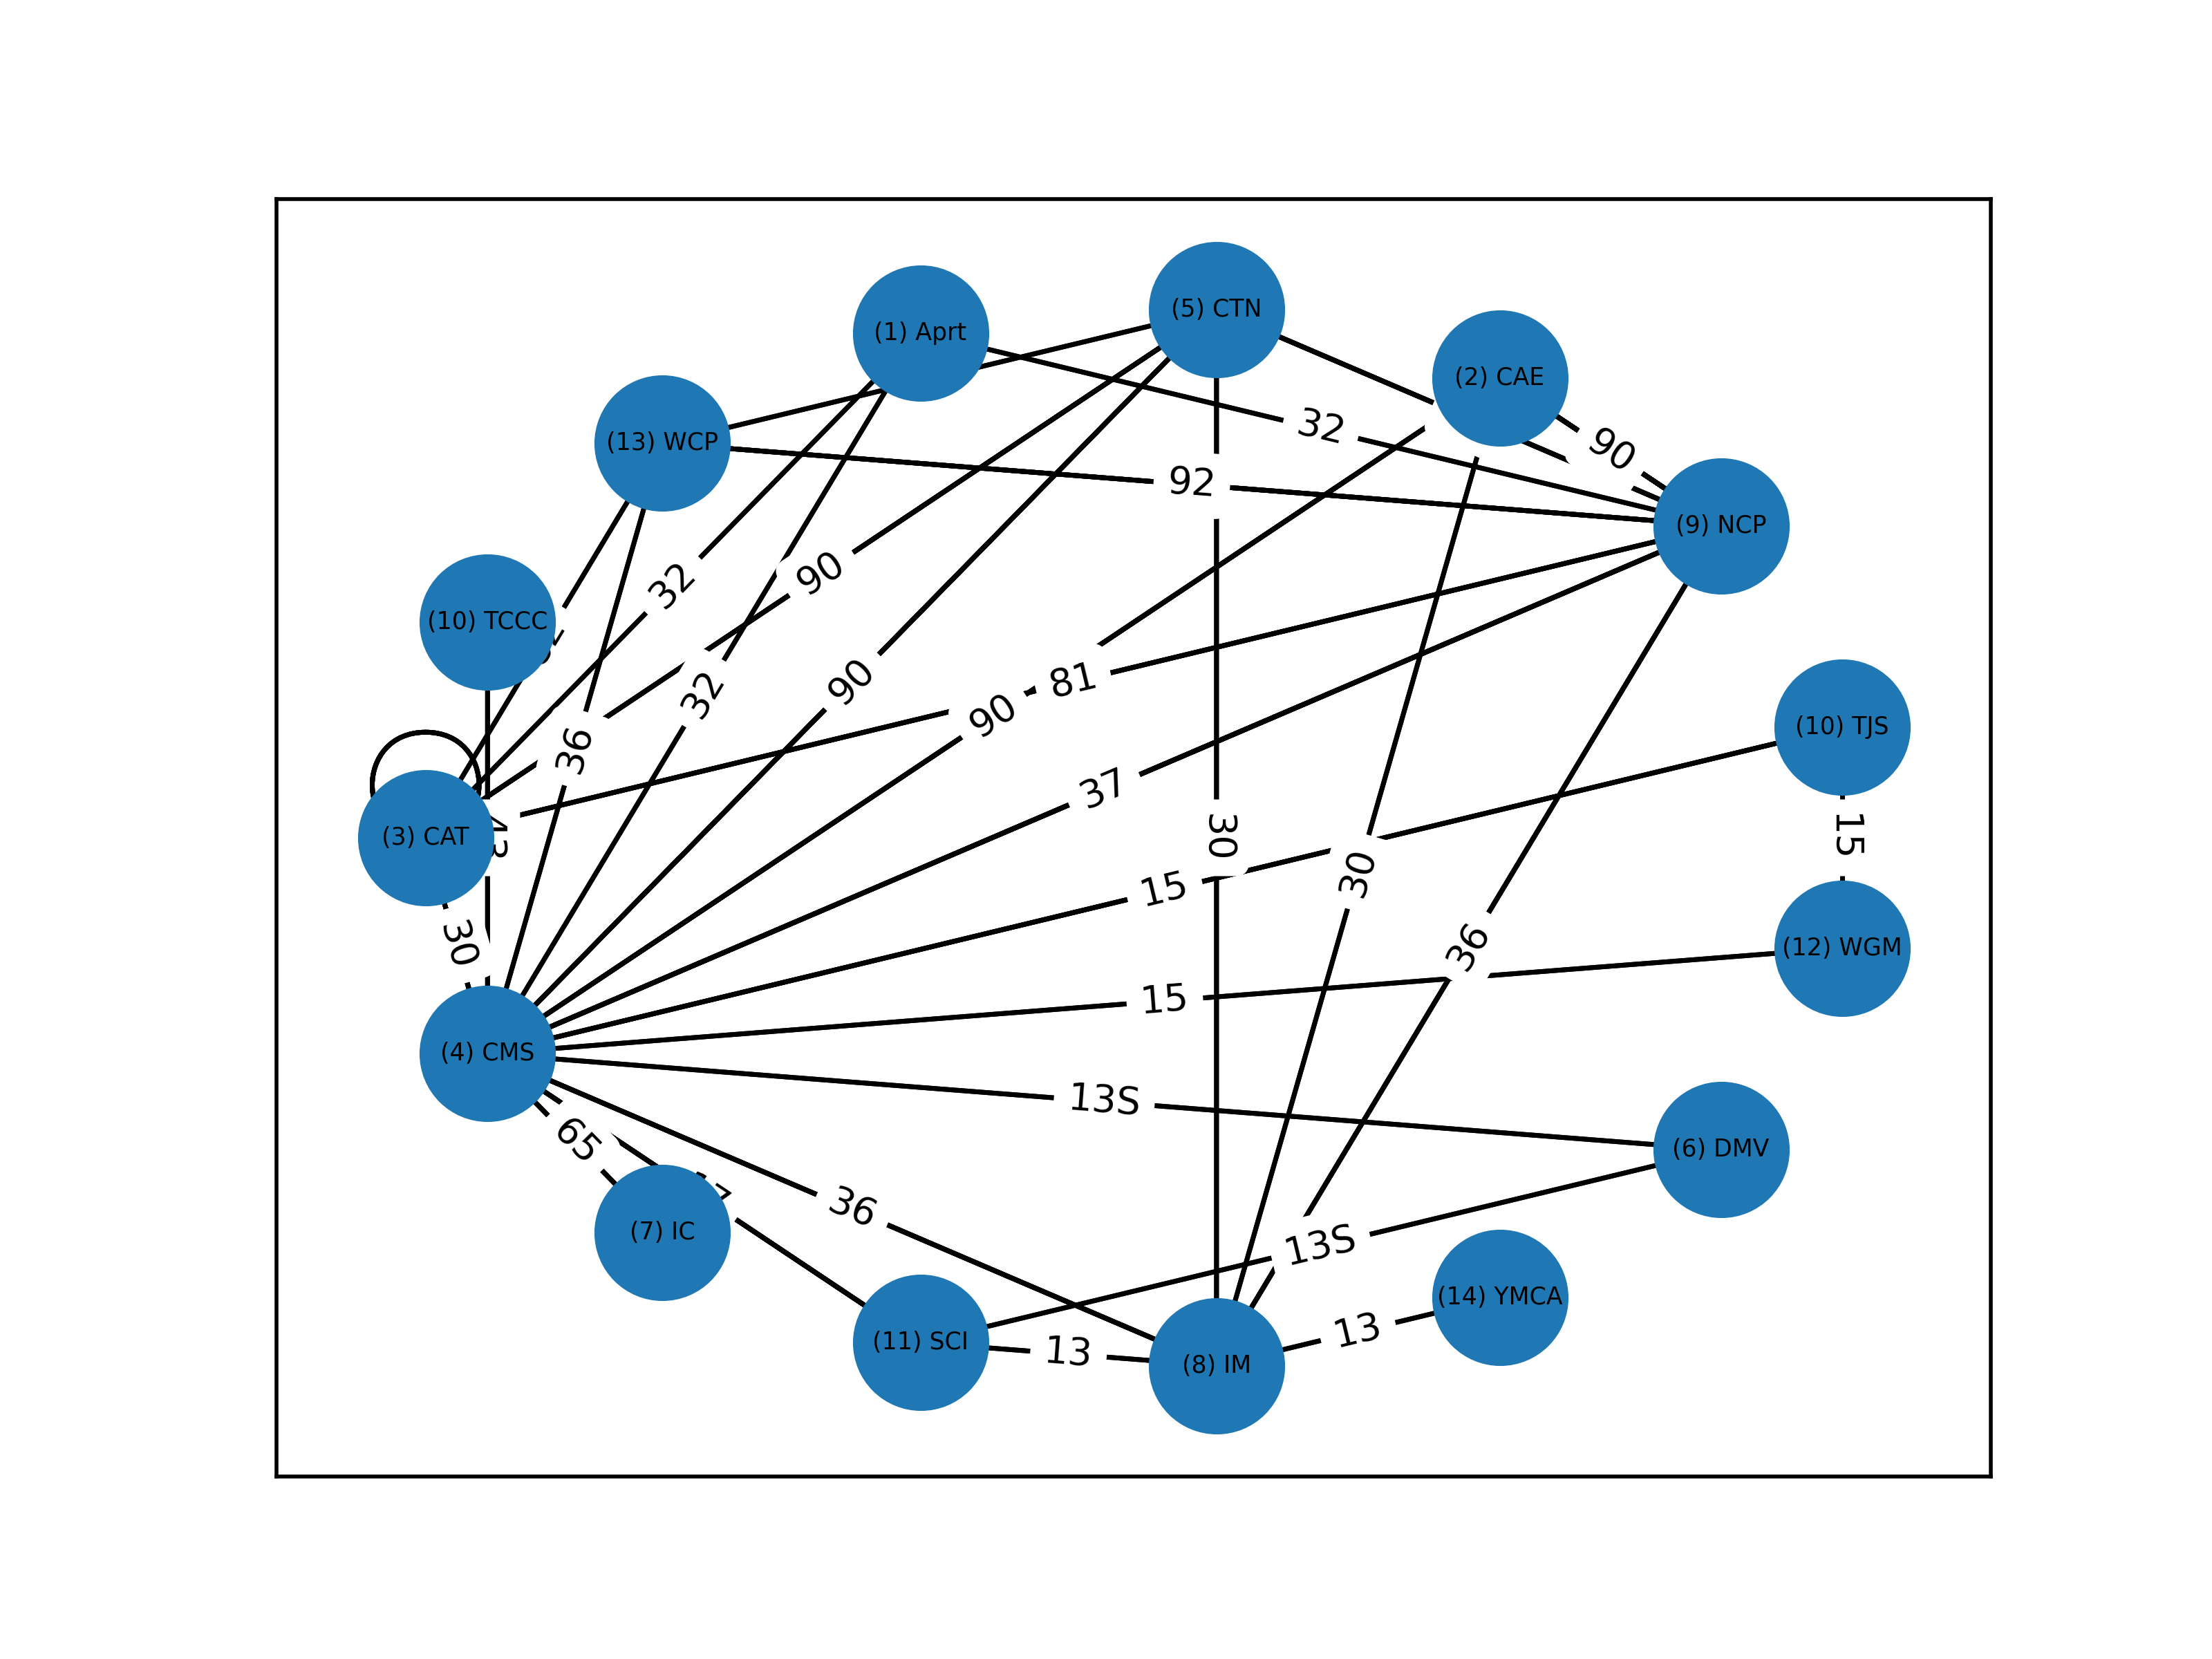
\includegraphics[width=6.5cm,height=6.5cm]{TCAT System Shell Layout.png}}}
\qquad\qquad
\begin{aligned}
L=
\begin{bmatrix} 
3&0&0&1&0&0&0&0&1&0\\
0&5&3&5&4&0&0&2&6&1\\
0&3&5&1&1&0&0&0&1&0\\
1&5&1&13&3&1&2&3&5&1\\
0&4&1&3&5&0&0&0&2&0\\
0&0&0&1&0&2&0&0&0&0\\
0&0&0&2&0&0&1&0&0&0\\
0&2&0&3&0&0&0&6&2&0\\
1&6&1&5&2&0&0&2&7&0\\
0&1&0&1&0&0&0&0&0&1\\
\end{bmatrix}
\end{aligned}
\]


\section {Fiedler Eigenvector, Eigenvalue, and Fiedler Set}
We understand visually that the network is complete, therefore no edges must be added. As such, the Fiedler value $\lambda_2=$ is greater than zero and the multiplicity of the eigenvalue of 0 is 1. We choose the first 10 nodes to calculate our value and vector simplicity of calculations.
\\ \\
Using the Julia programming language and an online compiler [3], we find that $\lambda_2=0.3660$ We also compute the corresponding Fiedler vector $v_2$ and list it below. 
\[
v_2=
\begin{bmatrix}
-0.089&
-0.12&
0.044&
0.28&
-0.06&
-0.17&
-0.89&
-0.09&
-0.05&
-0.25
\end{bmatrix}
\]
Accounting for all positive nodes in $v_2$, the resulting Fiedler set is as follows:
\[F=
\begin{bmatrix}
3 & 4
\end{bmatrix}
\]

\section{Analysis and Discussion}
The resulting split shows that only 2 of the 10 chosen locations were on the positive side of the split. Those two nodes, representing Central (Tower Rd.) and The Commons, make sense, as they are most frequented, and therefore served by many stops. The Commons, for example, have 13 routes going through it. Moreover, Tower Rd. of Central Campus remains a very popular location, as students transporting to and fro class often end up there, due to its central location to Cornell. We therefore see a large number of routes serving this stop.The locations with the most negative locations, Nodes 10 and 7, represent TC3 and Ithaca College, respectively. In making the graph, it is shown that these locations are only served by one or two routes, and these routes aren't as well connected to other popular locations. In essence, these locations are much more alienated to the network. 

We see a split between nodes, representing well-connected and not well-connected stops. This make sense in a real-world context, as the positive value nodes are popular by location. Places like downtown and the Cornell Campus will likely be more frequented than the YMCA or the DMV. However, it is surprising that there are so few positive fiedler values. This can be explained by the fact that these locations are more popular a far larger scale than the other stops - The Commons have nearly twice the amount of routes than the next highest served stop.

We see, then, the TCAT network of bus routes and locations in a visual and mathematical approach. It is obvious the most well-connected locations are the nodes with most amounts of edges, and vice versa is true. The fiedler values of each node represents how inter-connected a bus stop is. For those with a positive value, it is a "central location," that which is connected by many popular routes. The opposite is true for negative and lower values: these nodes are not well connected as they have fewer edges and smaller routes.

\section{Sources and GitHub}
1. \emph{About TCAT}, Tompkins Consolidated Area Transit Inc., 2022. https://tcatbus.com/about/about-tcat/\\
2. \emph{Popular Destinations}, Tompkins Consolidated Area Transit Inc., 2022. https://tcatbus.com/ride/popular-destinations/ \\
3. \emph{Online Julia Compiler}, Tutorials Point, 2022. https://www.tutorialspoint.com/execute\_julia\_online.php
\\ \\
This project, including the Python program, Julia script, and spreadsheets can be found on \href{https://github.com/Ming-DeMers/TCAT-Network-and-Fiedler-Set-Project}{GitHub here.} 

\end{document}
